\documentclass[preprint,footinbib,amsmath,amssymb,superscriptaddress]{revtex4}
\usepackage{graphicx,amsmath}
\usepackage{color}
\begin{document}
\draft


\title{Gelation as condensation frustrated by hydrodynamics and mechanical tension}
\author{Hideyo Tsurusawa}
\affiliation{ {Institute of Industrial Science, University of Tokyo, 4-6-1 Komaba, Meguro-ku, Tokyo 153-8505, Japan} }
%\thanks{These authors contributed equally to this work}
\author{Mathieu Leocmach}
\affiliation{Univ Lyon, Université Claude Bernard Lyon 1, CNRS, Institut Lumière Matière, F-69622, VILLEURBANNE, France}
%\thanks{These authors contributed equally to this work}
\author{Hajime Tanaka}
%\email{tanaka@iis.u-tokyo.ac.jp}
\affiliation{ {Institute of Industrial Science, University of Tokyo, 4-6-1 Komaba, Meguro-ku, Tokyo 153-8505, Japan} }

\begin{abstract}
{\bf A colloidal gel is an important non-ergodic state of matter, which can have elasticity and fluidity at the same time. Colloidal gels are known to be formed by phase separation accompanying dynamical arrest of a colloid-rich phase due to glass transition \cite{piazza1994phase,verhaegh1997,tanaka1999colloid,poon2002,lu2008gelation}. 
The presence of a liquid component should play crucial roles in the formation of a network structure and its time evolution, since it gives a constraint from the conservation of fluid momentum, which is known to affect the kinetic pathway of non-equilibrium phenomena \cite{tanaka2000viscoelastic}. However, there has so far been no experimental study on this important problem.  
Using a novel experimental protocol initiating phase separation, we successfully follow by confocal microscopy observation the entire process of gelation from the very beginning with a single-particle resolution   
and reveal the roles of hydrodynamics and mechanics in gelation, for the first time. 
%We switch off long-range Coulomb interactions between charged colloids by injecting salt at $t=0$ through an osmotic membrane and make depletion attractions due to polymers operative. This initiates phase demixing without inducing disturbing flow, which is inevitable for a conventional method, i.e., simple mixing of colloids and polymers at $t=0$. 
We show that hydrodynamic interactions between colloids mediated by a liquid component are the key to formation of a percolated network structure in  
a dilute system. Furthermore, the network formed by this mechanism is inevitably in a high energy state and under self-generated mechanical tension due to its connectivity. We find clear experimental evidence that network coarsening proceeds by sequentially repeating stress-driven mechanical fracture of a network strand. A stable gel is then formed when the network breaking rate becomes negligible. 
%Thus, we succeeded in clarifying the roles of momentum conservation, more specifically hydrodynamics and mechanics, in gelation, which has not been accessed experimentally. 
These findings provide an experimental basis for understanding the microscopic physical mechanism of gelation and its structural formation, whose kinetic pathway is selected not by a thermodynamics factor but by mechanical factors.}
\end{abstract}

\maketitle

%\section*{Introduction} 
Gels do not flow and behave as soft solids in a macroscopic scale, but have excellent fluid-like transport characteristics in a microscopic scale, 
which often provides essential functions of many biological gels including those in our body.  
For any gels, elasticity comes from the presence of a space-spanning percolated network that can transmit mechanical stress.
However, the network can be formed by different mechanisms: chemical reaction and physical processes such as phase separation. 
Gels spontaneously formed by phase separation are an important class of gels, which can be seen commonly in various soft matter \cite{tanaka2013phase} such as colloidal suspensions, emulsions, protein solutions, surfactant solutions, and polymer solutions, and now widely known as ``spinodal gels''.  This type of gels are not only of fundamental importance in physical, materials, and biological science, but also of technological importance in food, cosmetics, and medical industries. 

The mechanism of spinodal gelation has particularly been studied for colloidal suspensions since they can be regarded as a model system for other systems. Thanks to extensive studies in the past, we now have a reasonable physical picture: Gelation is induced by spinodal decomposition into two phases whose dynamics are very different \cite{tanaka1999colloid,tanaka2000viscoelastic} and the resulting vitrification of the slower phase \cite{piazza1994phase,verhaegh1997,tanaka1999colloid,poon2002,lu2008gelation}. 
However, the knowledge of ordinary spinodal decomposition cannot explain the observed behaviour since it predicts that the minority colloid-rich phase should form isolated clusters rather than a percolated network. This mystery was solved by using an analogy of phase separation of colloidal suspensions to that of polymer solutions on the basis of the concept of dynamic asymmetry \cite{tanaka1999colloid}. 
What is common in these two systems is that a mixture is composed of large slow components (colloid or polymer) and small fast components (solvent). 
On a macroscopic level, such dynamically asymmetric mixtures are known to show universal pattern formation, known as ``viscoelastic phase separation'' \cite{tanaka2000viscoelastic}. 
On a microscopic level, however, there are essential differences between colloidal suspensions and polymer solutions coming from the topological difference (sphere vs. chain), leading to 
distinct rheological behaviours. Thus there are many open questions about the elementary process of phase separation of colloidal suspensions and the resulting colloidal gelation.   
From the physical viewpoint, the presence of a fluid component indicates the importance of fluid momentum conservation in phase separation, which makes hydrodynamics and mechanics active in structural evolution. This is the key for viscoelastic phase separation \cite{tanaka1999colloid,tanaka2000viscoelastic}. There have been some numerical studies on the role of hydrodynamics~\cite{tanaka2000simulation,Furukawa2010} and mechanics~\cite{cipelletti2000universal,Tanaka2007,colombo2014self,testard2014intermittent} in colloidal gelation, however, there has so far been no experimental study that directly addresses these effects by dynamical observation of the process.  

%However, there have remained many open questions: (1) Spinodal decomposition usually form compact clusters (or, droplet) at low volume fractions where colloidal gels are formed, but actually it produces a space-spanning percolated network.  According to the common knowledge of ordinary phase separation, bicontinuous network can be formed only when the volume fraction is near 50 \%. (2) Even after forming a percolated network, i.e. a gel, structural evolution often slowly continues to proceed. This kind of ageing behaviour is quite important for a long-time stability of a gel state and a crucial problem in industries. (3) It is intuitively appealing that vitrification leads to dynamical arrest of spinodal decomposition and freezes the network structure of gels. But vitrification, or glass transition, is originally defined for bulk materials. On noting that the strands of a gel network are often very thin, and thus it is hardly clear whether we can apply the concept of glass transition as it is to describe dynamic arrest in gelation. 

To access these fundamental problems experimentally, we need to study the entire process of gelation from the beginning to the end at the single-particle resolution. 
Thus, confocal microscopy observation is necessary. However, it has been very difficult to study the very early and late stage of gelation by this method. 
Gelation of micron-size colloids suitable for quantitative confocal microscopy is usually induced by depletion attractions due to polymers in the solvent. 
%Polymers used for this purpose usually have high molecular weights because colloids have to be large enough for realizing particle-level resolution, which results in a high viscosity of the polymer solution. Ideally we want to switch on attractive interactions at $t=0$. But a high viscosity of a polymer solution prevents its rapid mixing with a colloidal suspension at $t=0$. 
The experimental protocols used so far for studying the kinetics of phase separation and gelation are as follows: (1) Colloidal suspensions and polymer solutions are mixed just before an experiment and after mixing transferred to a capillary tube as quick as possible. 
(2) A mixture, which is already in a final state point in the phase diagram and intrinsically unstable, or phase-separated, is vigorously mixed just before an experiment to break pre-existing phase separated structures by shear melting. 
However, these protocols have two common serious deficiencies: Firstly the initial state can never been homogeneous perfectly and there already exist particle aggregates at $t=0$. Secondly, the mixing inevitably involves 
turbulent flow, which does not decay but remain when the observation is initiated. 
Because of these intrinsic problems of the conventional protocols, it has been almost impossible to access the very initial stage of gelation without interference of pre-existing aggregates and/or turbulent flow.  
Strictly speaking, the gelation process observed by these conventional protocols inevitablly suffers from the influence of ill-defined initial static and dynamic conditions. 
%On the other hand, to access the late stage, we need to achieve a very accurate density matching to prevent gravitational effects and also a very accurate determination of coordinates of particles.  
%Now we review what has so far been known for the above open questions. On question (1), some time ago we proposed an explanation on the basis of the concept of viscoelastic phase separation. When the two components of a mixture have large size disparity and the resulting strong dynamic asymmetry, even the minority phase can form a percolated network structure. This is supported by numerical simulations using the viscoelastic model on the basis of an empirical constitutive relation \cite{tanaka2000viscoelastic}, however, how we can explain this at a microscopic level. We stress that there is no well-defined constitutive (stress-strain) relation for colloidal suspensions \cite{tanaka1999colloid}. We have studied numerically colloidal gelation by incorporating many-body hydrodynamic equation \cite{Furukawa2010} and showed the incompressibility of a fluid component prevents the formation of compact clusters but assists the formation of elongated clusters. However, there has been no experimental observation of the dynamical process of particle aggregation that shows a clear signature of the important roles of hydrodynamic interactions, although there is a work studying the characteristics of instantaneous cluster structures. However, we cannot deny a possibility that elongated clusters are formed not due to many-body hydrodynamic interactions, but rather by the above-mentioned turbulent flow induced by the conventional protocol. To reveal hydrodynamic effects in a convincing manner, thus, we need to study the dynamical process of particle clustering without any interference of perturbative flow.  On question (2), we have some numerical evidence for the important role of mechanical stress in network coarsening ~\cite{Tanaka2007,colombo2014self,testard2014intermittent}, but there has so far been no experimental evidence to our knowledge. On question (3), we need to clarify the relation between mechanical stress and yield stress. 
In this Letter, we study roles of hydrodynamics and mechanics in colloidal gelation experimentally by dynamical confocal microscopy observation of the entire gelation process from the beginning to the end with particle-level resolution. 
To access roles of hydrodynamics in the initial stage of gelation, we develop a new protocol to initiate phase separation without causing any harmful flow. 
To access roles of mechanics in the late stage, we realize a density matching of the order of 10$^{-4}$ (gravitational Peclet number $Pe< 10^{-6}$) and use a very accurate particle tracking method \cite{leocmach2013novel}. 
%In previous studies, the process of gelation has been studied experimentally by following the structural evolution. However, the roles of hydrodynamic interactions and mechanical stresses have never been addressed experimentally. 
These allow us to experimentally reveal (i) the importance of hydrodynamic interactions in forming and stabilizing elongated clusters and their percolation and (ii) the crucial role of mechanical stress 
in ageing of gels and a microscopic mechanism of the network breakup events. These findings will provide crucial information on the mechanisms of gel formation and coarsening and also 
on the fate of gels.  

%\section*{Results}

%\subsection*{System design}



We designed an experimental set-up that allows the observation of the entire process of gelation at a single particle level. For that, we use a colloidal system that is charge stabilised at long range, has a short range depletion attraction, and is also sterically stabilised causing nearly hard sphere repulsion at contact. We disperse colloidal particles and non-adsorbing polymers in a  mixture of organic solvents that matches both the refractive index and the density of the particles. Because of the weakly polar nature of the solvent mixture (its dielectric constant $\epsilon_r = 5\sim6$), the Debye screening length is about $\kappa^{-1}=10$ $\mu$m, long enough for the large colloids (diameter $\sigma=2.75$ $\mu$m) to form a homogeneous Wigner crystal in the mixture~\cite{klix2010structural}, since the short ranged ($\sim \sigma/10$), depletion attraction caused by the polymers is masked by the electrostatic repulsion.

We enclose the suspension in a thin microscopy cell sketched in Fig.~\ref{fig:cell_vs_cap}a. The bottom wall of the cell is an osmotic membrane providing contact with a long channel full of the same solvent mixture. We introduce solid salt at the other end of the channel. Salt dissolution and subsequent migration of the ions along the channel and through the membrane induce screening of the electrostatic repulsion, revealing the depletion potential well due to the pre-existing polymers. The time needed for the ions to diffuse from the membrane across the cell thickness is of the same order of magnitude as the Brownian time of the particles $\tau_B=10$ s. This method causes uniform gelation starting from the homogeneous Wigner crystal state without any solvent flow, allowing \textit{in situ} confocal microscopy observation throughout the process from $t \sim 0$.

As noted above, the conventional shaking or shear melting protocols for the initiation of phase separation cause severe non-ideal perturbation to a system. To show this,  
we compare, in Fig.~\ref{fig:cell_vs_cap}b and c, confocal microscopy images of the final structures for two gels prepared at the same state point: one by our protocol and the other by introducing in a capillary an existing gel and thus shear melting it, respectively. The later is coarser, highlighting that shaking or shear melting protocols~\cite{lu2008gelation,Teece2011,Bartlett2012} are not equivalent to a quench. 
Our novel quench protocol provides an ideal experimental platform to make a comparison with theory and simulations. However, we note that Brownian Dynamics simulations cannot reproduce our experimental results even with the same quench, because of the lack of a solvent mediating hydrodynamic interactions~\cite{tanaka2000simulation,Furukawa2010}. 
%Thus our protocol might be very close to application relevant processes where the sudden addition of a component (e.g. salt, acid, depletion agent) induces aggregation in an otherwise stable suspension (e.g. milk).

In Fig.~\ref{fig:cell_vs_cap}d, we show a computer reconstruction from experimental coordinates of a typical gelation experiment at a relatively low volume fraction ($\phi=7.5\%$). Immediately before ions enter the cell ($t=0$), the suspension is in a Wigner crystal state where the particles are far apart due to long range Coulomb repulsion. As soon as the charges are screened, the particles begin to aggregate and form clusters that progressively connect to each other while coarsening to finally percolate over the field of view around $t=35$ min.

%\subsection*{Observation of the initial stage}

In Fig.~\ref{fig:phasediag}a, we show the phase diagram, where we can divide the state points into three regions based on the final state obtained by our protocol: at low polymer concentration ($c_p<0.2$ g/$\ell$) a sample fully relaxes to a fluid state; at very low colloid volume fraction ($\phi<0.05$) and high polymer concentration the particles condense into long-lived well separated clusters as observed in~\cite{Lu2006}; in the rest of the explored phase space we observe a long-lived space spanning network. 
We also show the theoretical spinodal line obtained by generalised free volume theory~\cite{Fleer2008}, which is in good agreement with our experimental points 
(the small discrepancy at small colloidal volume fractions is common in free volume theory~\cite{Shah2003,Bergenholtz2003,lu2008gelation}). 

With our technique we can observe the entire kinetic path leading to the final state at a single-particle level. To characterise this path, we compute the instantaneous mean number of neighbours $\bar{N}_C$, or coordination number that quantifies the compactness of the structure. We also compute the the spatial extent of the largest cluster $l_\text{max}$ that we normalize by the size of the field of view $L$ to obtain a measure of the distance to percolation of the system. Figure~\ref{fig:phasediag}b shows a system trajectory in the $(l_\text{max}/L, \bar{N}_C)$ plane for various colloidal volume fractions. At high densities, percolation takes place first, within the first few $\tau_B$ after charge screening by salt, and then coarsening proceeds. At low densities, percolation never takes place and we observe the compaction of individual clusters. In between, we observe the process detailed in Fig.~\ref{fig:cell_vs_cap}d: formation of low-compacity clusters that then slowly connect together to build the percolating network. This process can take hundreds of $\tau_B$ and is competing with cluster compaction, as indicated by the oblique trajectory (red open circles) in Fig.~\ref{fig:phasediag}b. The path to gelation in this plane is thus not universal and depends on the colloid volume fraction even within the gelation region.

The initial similarity between the trajectories of dilute gels and cluster phase is striking, as if their dynamics were ruled by the same phenomenon. To confront this hypothesis, we compute the time dependent static structure factor $S(q,t)$. For all gel and cluster samples, we observe the appearance of a low $q$ peak in $S(q)$, see Supplementary Figure~1, which is characteristic of spinodal decomposition in a system of a conserved order parameter. To track the position of this peak, we compute the characteristic wave number $\langle q \rangle$ and show its temporal evolution in Fig.~\ref{fig:phasediag}c. The curves for all samples follow a master curve coherent with spinodal decomposition kinetics: At short times $\langle q \rangle(t)$ shows a plateau indicating that the low $q$ peak builds up at constant wave number corresponding to distances of about $2\sigma$. This plateau is characteristic of the early stage spinodal decomposition, which is described by Cahn's linear theory \cite{onuki2002phase}. At intermediate times, on the other hand, we observe coarsening with \textcolor{blue}{$\langle q \rangle \sim t^{-1/2}$, which is often observed in viscoelastic phase separation 
(see, e.g., \cite{Furukawa2010}).} Finally at longer times each sample deviates from the master curve to form a plateau indicating arrest. The more dilute samples arrest sooner, 
but the origin of arrest is different between clusters and percolated networks. For clusters, density fluctuations grow rather rapidly in the initial stage, but after the formation of isolated clusters their growth takes a long time since the diffusive evaporation-condensation mechanism does not work for colloidal viscoelastic phase separation and direct cluster collisions and coalescence are necessary for coarsening \cite{tanaka2000viscoelastic}. For networks, densification due to phase separation leads to dynamic arrest due to vitrification \cite{piazza1994phase,verhaegh1997,tanaka1999colloid,poon2002,zaccarelli2007,lu2008gelation} or formation of locally stable structures \cite{royall2008g}. 
Our observations indicate that both cluster and gel phases are due to viscoelastic spinodal decomposition: network-type spinodal for the gel, and droplet-type spinodal for the clusters where strong dynamical asymmetry between colloids and the solvent leads to unique roles of hydrodynamics and mechanics in phase separation \cite{tanaka1999colloid,tanaka2000viscoelastic}.

Here two questions remain, corresponding respectively to the dilute or dense routes to gelation: (i) How can individual clusters percolate a long time after their formation? (ii) How does a percolated network evolve toward more compact states? We will show that the answers come from mechanical effects: respectively hydrodynamics and internal mechanical stresses.

%\subsection*{Role of hydrodynamics}

First we focus on the role of hydrodynamics. 
In Fig.~\ref{fig:hydro}a, we follow the compaction of clusters made of only three particles in a non-percolating sample. The probability distribution of the radius of gyration $R_g$ of these triplets shows two peaks on both sides of $R_g^*=0.8\sigma$. For $R_g<R_g^*$ the cluster is compact, with a structure close to an equilateral triangle. For $R_g>R_g^*$ the three particles are aligned and the cluster is elongated. We found that just after the quench most triplets are elongated and then either connect to other clusters or relax to the more stable compact state. To follow this relaxation, we define the probability to stay elongated as
\begin{equation}
P_\text{el}(\Delta t) = \left\langle P\left(\delta_i(t+\Delta t)|\delta_i(t)\right)\right\rangle_{t,i}, 
\end{equation}
where $\delta_i(t)$ is the probability for the triplet $i$ to be elongated at time $t$. The decay of $P_\text{el}(\Delta t)$ has a characteristic time of $27\tau_B$, much longer than the Brownian time. 

The shape of clusters of more than 3 particles cannot be followed in the same way. Thus we compute the principal moments of gyrations $\lambda_j$ with $\lambda_1\geq\lambda_2\geq\lambda_3$. Low values of the aspect ratios $\lambda_2/\lambda_1$ and $\lambda_3/\lambda_1$ indicate that the cluster is flat or even linear. In Fig.~\ref{fig:hydro}b, we show the evolution of the average value of these aspect ratios either for a non-percolating sample or before percolation for a percolating one. In both cases, we observe that the clusters are originally not compact and become more isotropic over tens of $\tau_B$. As can be seen in Fig.~\ref{fig:cell_vs_cap}d, structural isotropy is recovered only after the fusion of many anisotropic clusters into a branched structure. 

These observations can be rationalised by the invocation of hydrodynamic effects. Indeed in a solvent, particles cannot converge freely to form compact structures~\cite{tanaka1999colloid,tanaka2000simulation,Furukawa2010}. The compaction is delayed by the incompressibility of the solvent, which allows only divergence-free transverse flow fields.  Furthermore, clusters influenced by hydrodynamic interactions tend to be more elongated, less compact. We can test this hypothesis by measuring at which angle particles meet relative to existing neighbours. If influenced by hydrodynamics, particles should avoid the direction of existing neighbours and come from more open angles.

In Fig.~\ref{fig:hydro}c we show the bond angle distribution from three points of view: (i) existing bonds, (ii) bonds that will form within the next $\tau_B$, (iii) bonds that will form within the next $\tau_B$ involving an isolated particle. As expected, existing bonds are preferentially at a 60$^\circ$ angle indicating stable packing, with secondary peaks coherent with a mixture of tetrahedral and hexagonal packings. Future bonds have more acute angles and almost never 180$^\circ$, since they are mostly due to particles attached to second neighbours, see sketch in Fig.~\ref{fig:hydro}c. Here hydrodynamics plays no role. By contrast, future bonds involving isolated particles form at more obtuse angles, with a clear peak around 180$^\circ$. This confirms that hydrodynamics influences particle aggregation and explains why clusters are initially elongated.

Consequently, long-lived elongated clusters have a higher probability to meet via either rotational or translational diffusion than compact spherical clusters. In Supplementary Figure~\ref{fig:effectiveVF} we show that indeed at all colloidal volume fraction percolation takes place when the effective volume fraction $\phi_\text{eff} = \sum\frac{4\pi}{3}R_g^3$ of the clusters reaches random close packing. Hydrodynamics explains why in a rather dilute regime we can observe immediate formation of elongated clusters and then their slow, hydrodynamically-assisted aggregation into a percolated structure.
We stress that this is a direct consequence of large-size disparity, which leads to the physical situation where discrete solid objects are floating in a continuum liquid. 

%\subsection*{Network ageing}
In the above, we show that with a help of hydrodynamic interactions, particles first form
a transient gel even at very low volume fractions, and thus only later they increase the number of
nearest neighbours to minimize the energy of the structure. 
Thus, hydrodynamic interactions lead to the formation of gels that are very far from equilibrium and under a strong thermodynamic driving force 
towards more stable compact structures. 
Due to the connectivity of the network, the resulting transition from open to more compact networks can take place only through
the breaking of the bonds that have accumulated more stress. The process was called stress-driven ageing~\cite{Tanaka2007}, 
which is characteristic of viscoelastic phase separation \cite{tanaka2000viscoelastic}. 
As we saw in Fig.~\ref{fig:phasediag}c, the coarsening in these samples is indeed much slower than what is expected from ordinary spinodal decomposition dynamics \cite{onuki2002phase}, 
suggestive of mechanical frustration effects. The phase separation is arrested, but the system is still ageing slowly, a process sometimes leading to delayed sudden collapse of gels~\cite{poon1999delayed,Bartlett2012}, a catastrophic phenomenon from the industrial point of view. Previous numerical studies~\cite{Tanaka2007,colombo2014self,testard2014intermittent} have shown that the main coarsening mechanism is the rupture of strands in the network, a process that to our knowledge has not been followed experimentally at the particle level.
Below we provide the first experimental proof of this process. 

Figure~\ref{fig:breaking}a shows a strand rupture reconstructed from confocal 3D images, the colours mapping the intensity of internal stresses acting on each particle. In practice, the attraction potential well is too narrow relative to the particle localisation errors for us to extract directly the force acting on a particle. Therefore, we use the elongation of the particle neighbourhood as a proxy. The more the bonds around a particle are oriented along a single axis, the more tension is exerted on the particle. This local elongation is quantified using bond orientational order~\cite{steinhardt1983boo} for the 2-fold symmetry $q_2$, see Methods for a precise definition. In Fig.~\ref{fig:breaking}a we observe the slow build up of tension over the first 30 min, until the tension is concentrated on a weak part, a one particle thin strand. This strand breaks and the particles involved merge in their respective part of the network that then stay apart from each other. This is the only elementary process allowed for a percolated network to lower the free energy and it is a mechanically driven coarsening process \cite{Tanaka2007}. The driving force is simply attractive interactions between particles favouring compact structures, which can be rephrased by 
interfacial energy in a coarse-grained picture. 

To detect strand rupture, we use the topology of the bond network. We can consider the gel as a graph with the particles as nodes and the bonds as edges. This graph evolves from frame to frame separated by $3\tau_B$. In the lower part of Fig.~\ref{fig:breaking}a, we draw in red the shortest on-graph path between two particles of interest. Before the strand rupture, this path is a single bond long. After the rupture, the shortest path is much longer. In general, when two particles were bonded on the previous frame and are no more bonded on the present frame, we define the post-breaking topological distance $\Lambda$ as the new shortest distance on the graph between them, minus 1. If the particles still have a common neighbour then $\Lambda=1$, because two bonds are needed to go from one to the other. $\Lambda=2$ when three bonds are needed, etc.

This path length $\Lambda$ is a good measure of the significance of a bond breaking event. Small values indicate a local rearrangement whereas large values are the signature of important changes in the topology of the network, namely strand rupture. Figure~\ref{fig:breaking}b shows the distribution of $\Lambda$ for three colloidal volume fractions. Excluding the largest values that are dominated by the limited size of the field of view, $\Lambda$ seems to follow a power-law distribution of exponent between $-3$ and $-4$. However the values at $\Lambda=1$ seems in excess. Figure~\ref{fig:breaking}c compares the probability distribution of $q_2$ for all bond breaking events versus for evens with $\Lambda>1$. In both cases bonds about to break have a higher probability of being under tension, but this trend is much clearer when excluding local events. Both observations point to spurious detection of bond breaking events due to localisation errors comparable to the short attraction range and rattling of particles. For this reason, but also to focus on topologically relevant strand rupture, we discard all events with $L \leq 3$ in the following analysis.

In Fig.~\ref{fig:breaking}d we show the time evolution of the probability for a topologically relevant strand rupture $P_\text{break}(\Lambda>3)$, i.e. the ratio of the number of bond breaking events with $\Lambda>3$ by the number of particles. $P_\text{break}$ has its maximum at percolation and then decreases and finally saturates. Strikingly all curves collapse after percolation, indicating common physical ingredients for the ageing of gels at all concentrations.

Initially, clusters are in elongated, unstable configurations. When isolated, a cluster is able to relax to a more compact and stable shape. However in dense samples, elongated clusters meet, before any compaction, into large branched clusters able to transmit stresses. The compaction trend exerts internal stresses on the strands inside those clusters large enough to make them rupture. This effect is maximum when the sample is fully percolated and thus the network is most strongly stretched, and the internal stresses are maximum.

The characteristic size of a spinodal network is \textcolor{blue}{$\xi(t)\sim t^{1/2}$} (see Fig. 2c). Strands being linear objects, their volume is linear in $\xi$ and thus the number of strands in the field of view $N_s$ evolves as \textcolor{blue}{$t^{-1/2}$}. Since after the percolation no new strands are to be created, the variation in the number of strands is given only by the strand rupture rate:
\begin{equation}
\textcolor{blue}{P_\text{break} = -\frac{d N_s}{dt} \sim t^{-3/2}.}
\end{equation}
Indeed in Fig.~\ref{fig:breaking}d we observe that the initial regime of the master curve is well described by a power law of exponent \textcolor{blue}{$-3/2$}. 
\textcolor{blue}{The saturation of $P_{\rm break}$ at late times may be an artefact due to a choice of $\Lambda$ too small for characterising breaking events taking place in the late stage. 
The criterion $\Lambda>3$ is good for the initial stage, but may be too strict for the late stage and detect local rearrangements. 
Thus, $P_{\rm break}$ should actually be negligible in the very late stage and the structure evolution is arrested (see Fig. 2c).} 
At longer times, most of the internal stresses have been released and the system reaches arrested phase separation, where the yield stress emerging due to dynamical arrest 
exceeds the internal mechanical stress. 
For dilute samples, percolation happens later, after the end of the power law regime. Thus, the clusters have already compacted to stable configurations and internal stresses are low.




% \section{Conclusion}
To summarize, we successfully follow the entire process of colloidal gelation at a single particle level and 
show that spinodal gelation is induced by spinodal decomposition, but the process is heavily frustrated  by 
hydrodynamics and mechanics, both of which originates from the dynamical asymmetry due to the large size disparity between 
colloidal particles and solvent molecules. The hydrodynamic effect is the consequence of the fact that solvent molecules 
can be treated as a continuum fluid in the much larger length and time scales of colloids and thus obey the Navier-Stokes equation. 
We can preclude a possibility that the formation of elongated clusters is due to non-ideal flow induced by the mixing, which may be the case for the conventional protocols. 
In a dilute system, local condensation proceeds simultaneously as percolation.
In contrast, dense systems accomplish percolation in the early stage, whereas local condensation proceeds in the late stage; and this rapid percolation leads to high internal stress at the time of percolation. 
In both cases of gelation, percolation is a consequence of condensation frustrated by hydrodynamic interactions, whereas the coarsening process is frustrated by mechanical tensions.
We also find that the fate of a percolated network, more specifically, whether it is permanently stabilised as a gel or eventually breaks up into isolated clusters, 
crucially depends on whether the weak parts of the gel network can support the self-generated mechanical stress or not. 
%In the systems studied the rate of the network breakup events decreases with time, but tends to remain finite even after 10$^3$ $\tau_{B}$, 
%suggesting that network may eventually loose its connectivity. 
Since colloidal suspensions can be regarded as an ideal model system of binary mixtures that consist of small and big components, 
our study will shed new light on not only colloidal gelation but also dynamically asymmetric mixtures, which include polymer solutions, emulsions, and protein solutions. 
We hope that our findings will deepen our microscopic understanding of spinodal gelation concerning the lower bound of gelation and the long-term stability, both of 
which are important in industrial applications.   


\section*{METHODS}

\subsection*{Experimental.}

We used \textsc{pmma} (poly(methyl methacrylate)) colloids sterically stabilized with methacryloxypropyl terminated \textsc{pdms}(poly(dimethyl siloxane)) and fluorescently labelled with rhodamine isothiocyanate chemically bonded to the \textsc{pmma}. Colloids are dispersed in a mixture of cis-decalin (Tokyo Kasei) and bromocyclohexane (Sigma-Aldrich) that matches both optical index and density of the colloids.

To induce short-ranged depletion attraction, we use polystyrene (TOSOH) of molecular weight 8.4$\times 10^6$ as non-adsorbing polymer. The radius of gyration in theta solvent is estimated to 110 nm. Here the solvent may be regarded as ``good'' and a Flory scaling of the measurements of~\cite{lu2008gelation} yields $R_g=148$ nm. In the absence of salt, the Debye length is expected to reach several $\mu$m and the (weakly) charged colloids experience a long range electrostatic repulsion~\cite{Royall2003}. We confirm that colloids never come close enough to feel the short-ranged attraction and form a Wigner crystal.

The colloids and polymers are contained in an observation cell ($10$ mm$^2$ $\times$ 200 $\mu$m) made of glass in contact with an half-open glass channel approximately 400 times larger in volume, via a millipore filter with pore size of 100 nm that allows the salt through but neither polymer nor colloid (see Fig.~\ref{fig:cell_vs_cap}a). The channel is filled with the same solvents at density matching composition. At the beginning of the experiment, solid tetrabutylammonium bromide (Fluka) is introduced to the channel. Data acquisition starts within 30 s after salt introduction. Our procedure induces practically no solvent flow in the observation cell. We confirmed the presence of undissolved salt several days after mixing, indicating that the observation cell was brought to saturation concentration.

Given the diffusion constants of Bromide and alkyl cation ($6$ and $2 \times 10^{-10}$~m$^2$/s~\cite{Campbell2005}), we estimate the characteristic diffusion time of salt from top to bottom of the order of 10~s. Therefore, we reach uniform final salt concentration into the observation cell within only a few Brownian times of the colloids. Indeed we measured a delay of about 1 min between the aggregation at the bottom and at the top of the cell. We define the initial time of the aggregation process when the maximum of the $g(r)$ jumps from the lattice constant of the Wigner crystal to the hard-core diameter $\sigma$.


We collect the data on a Leica SP5 confocal microscope, using 532 nm laser excitation. The temperature was controlled on both stage and objective lens, allowing a more precise density matching. The scanned volume is at least $82 \times 82 \times 85$~$\mu$m$^3$. The particle coordinates are tracked in three dimensions (3D) with an accuracy of around $0.03\sigma$~\cite{LeocmachColloids}.

\subsection*{Analysis.}

From direct confocal measurements~\cite{Royall2007, Poon2012}, we estimate the hard-core diameter of our colloids ($\sigma=2.75$~$\mu$m) and the range of the interaction potential (that confirmed our scaling of $R_g$ within $1\%$), leading to a polymer-colloid size ratio $q = 2R_g/\sigma = 0.10(6)$. Spinodal line on Fig.~\ref{fig:phasediag}b are calculated from this size ratio using the generalized free volume theory~\cite{Fleer2008}.

In principle the attraction well of the depletion extends to $\sigma+2R_g$, however, resolution-dependent tracking imprecisions and systematic errors do not give a precise enough estimate of such short distance. Therefore we consider two particles bonded when their distance is shorter the first minimum of $g(r)$, i.e. 3.55~$\mu$m. This defines the bond graph that we analyse using connected components and shortest path analysis algorithms~\cite{Hagberg2008}.


To detect local 2-fold symmetry and thus elongation, we use \citet{steinhardt1983boo} bond orientational order for the particle $i$,
\begin{align}
	q_2(i) =& \sqrt{\frac{4\pi}{5} \sum_{m=-2}^{2} |q_{2,m}(i)|^2 }, \label{eq:ql}\\
	q_{2,m}(i) =& \frac{1}{N_i}\sum_{j=1}^{N_i} Y_{2,m}(\theta(\mathbf{r}_{ij}),\phi(\mathbf{r}_{ij})),
	\label{eq:qlm}
\end{align}
where the $Y_{\ell, m}$ are spherical harmonics and $\mathbf{r}_{ij}$ is one of the $N_i$ bonds involving particle $i$.

\bibliographystyle{naturemag3}
\bibliography{ico_dyn}

\vspace{1cm}
%\item[Supplementary Information] is linked to the online version of the paper at www.nature.com/nature.
\noindent
{\bf Acknowledgements.} This study was partly supported by Grants-in-Aid for Scientific Research (S) (Grand No. 21224011) and Specially Promoted Research (Grand No. 25000002) from 
the Japan Society for the Promotion of Science (JSPS). 

%\vspace{0.3cm}
\noindent
{\bf Author Contributions.} H.Ts. and M.L. contributed equally to this work. 
H.Ta. conceived and supervised the project, H. Ts. performed experiments, M.L. analysed the data, and all authors discussed and wrote the manuscript. 

%\vspace{0.3cm}
\noindent
{\bf Author Information} Reprints and permissions information is available at www.nature.com/reprints.
Correspondence and requests for materials should be addressed to H.T. ~(tanaka@iis.u-tokyo.ac.jp).

\clearpage
\begin{figure*}
	%\includegraphics[width=16cm]{figure1.pdf}
	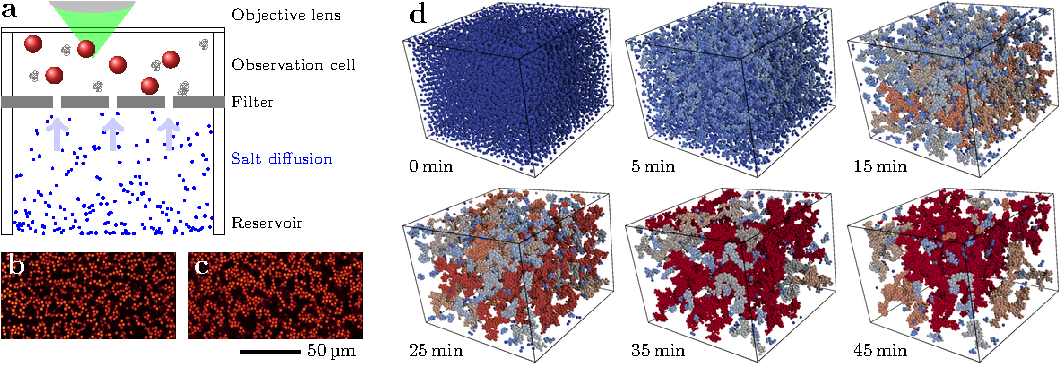
\includegraphics{figs/cell_vs_cap2.pdf}
	\caption{\textbf{Reservoir cell.} \textbf{a,} Sketch of our experimental setup. The observation cell contains initially colloids, polymer and no salt. \textbf{b,} Confocal slice of a gel formed \textit{in situ} by our method ($\phi=25.5~\%$, $c_p=1.4$ g/$\ell$), 1 hour after gelation. \textbf{c,} Idem for a gel at the same state point formed \textit{ex situ} and immediately pumped into a capillary. \textbf{d,} Gelation observed by our method. Experimental coordinates are reconstructed and coloured by the number of particles in clusters in a typical sample close to the cluster-gel line ($\phi=7.5~\%$, $c_p=1$ g/$\ell$). Origin of time is the last frame before melting of Wigner crystal.
	%Phase diagram obtained in reservoir cell. Spinodal line is obtained from free volume theory. State points analysed in the text are circled. The state point of \textbf{b-c} is highlighted by a square.
	}
	\label{fig:cell_vs_cap}
\end{figure*}

\clearpage 
\begin{figure}
%\includegraphics[width=10cm]{figure2.pdf}
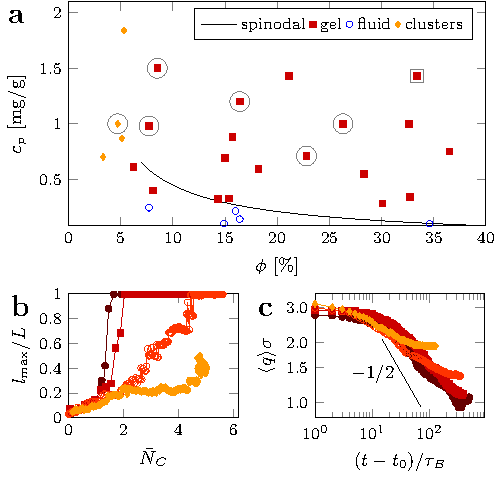
\includegraphics{figs/phasediag.pdf}
\caption{\textbf{Different regimes of gelation.} \textbf{a,} Phase diagram. Experimental points are categorised based on the final state obtained in reservoir cell. The spinodal line is obtained from free volume theory. State points analysed in the text are circled. The state point of Fig.~\ref{fig:cell_vs_cap}b-c is highlighted by a square. \textbf{b,} Comparison of system evolution in terms of largest cluster extent and of mean coordination number. By increasing density: $\phi=4.2,\,8,\,16,\,27~\%$, $c_p=1,\,1.5,\,1.2,\, 1$ g/$\ell$ for 
%\textcolor{red!40!yellow}
{$\blacklozenge$}, 
%\textcolor{red!80!yellow}
{$\circ$}, 
%\textcolor{red!80!black}
{\tiny$\blacksquare$} and 
%\textcolor{red!40!black}
{$\bullet$} respectively. \textbf{c,} Growth of the characteristic wave number for the same samples. 
The line is a scaling law for the intermediate coarsening regime for network-forming phase separation.}
\label{fig:phasediag}
\end{figure}

\clearpage
\begin{figure}
	%\includegraphics[width=10cm]{figure3.pdf}
	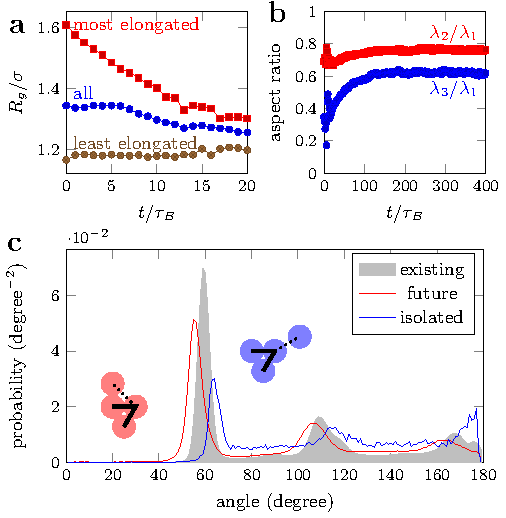
\includegraphics{figs/hydro.pdf}
	\caption{\textbf{Hydrodynamics} \textbf{a,} Probability of staying elongated for a triplet in a non-percolating sample ($\phi=4~\%$, $c_p=1$ g/$\ell$). The continuous line is the best exponential fit of characteristic time $27\tau_B$. Inset: probability distribution of radii of gyration of triplets. \textbf{b,} Evolution of the aspect ratios of clusters of 4 particles and more in the same sample (dashed lines) and in a percolating sample ($\phi=8~\%$, $c_p=1.5$ g/$\ell$, continuous lines). \textbf{c,} Bond angle distribution relative to existing bonds (gray), to a future bond (red) or to a future bond involving an isolated particle (blue) obtained in the percolating sample. Future bonds are shifted to smaller angles, whereas gas adsorption takes place from larger angles. Insets sketch both cases, with present bonds drawn thick and future bonds drawn dotted.}
	\label{fig:hydro}
\end{figure}

\clearpage
\begin{figure*}
%\includegraphics[width=16cm]{figure4.pdf}
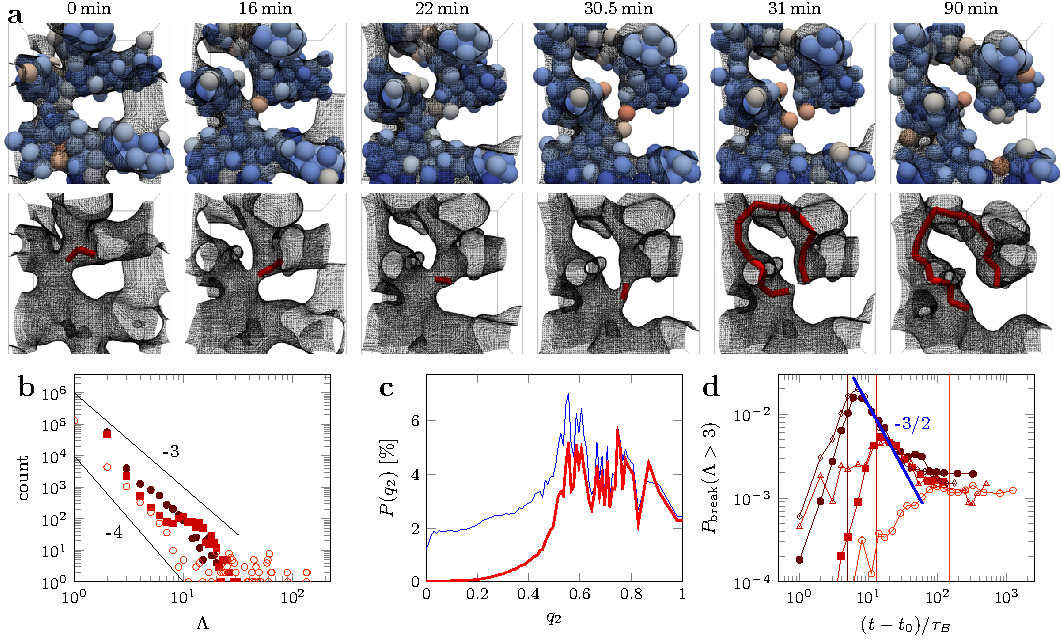
\includegraphics{figs/breaking.pdf}
\caption{\textbf{Mechanical tension drives coarsening} 
\textbf{a,} Reconstruction from experimental coordinates ($\phi=29~\%$, $c_p=0.7$ g/$\ell$) of coarsening process geometry (top) and topology (bottom). Particles are drawn to scale and coloured by $q_2$ from blue (low) to red (high). The meshed surface is a Gaussian coarse-graining of the network pattern. The red line indicates the shortest on-graph path between the two particles of interest. 
\textbf{b,} Number of bond breaking function of the future on-graph distance $\Lambda$ (after percolation) for the three percolating state points of Fig. 2a (same colours and markers).
%three state points of increasing density: $\phi=8,\,16,\,27~\%$, $c_p=1.5,\,1.2,\,1$g/$\ell$ for \textcolor{red!80!yellow}{$\circ$}, \textcolor{red!80!black}{\tiny$\blacksquare$} and \textcolor{red!40!black}{$\bullet$} respectively.
\textbf{c,} Probability for a bond to break during $3\tau_B$ function of bond-centred $q_2$ for all events (blue) and for events with $\Lambda>1$ (thick red) in the same sample as \textbf{a}.
\textbf{d,} Evolution of the topologically relevant bond breaking probability ($\Lambda>3$) for the same state points as in b. Vertical lines indicate the respective percolation times.
}
\label{fig:breaking}
\end{figure*}

\end{document}